% small.tex
\RequirePackage{atbegshi}

\documentclass{beamer}
\usetheme[height=7mm]{Rochester}

\usepackage{graphicx}
%\usepackage{movie15}
\usepackage{hyperref}
\usepackage{skull}
\usepackage{verbatim}
\usepackage[utf8]{inputenc} 
\usepackage[T1]{fontenc}
\usepackage[czech,english]{babel}

\title{Autíčko + webkamera + neuronová síť = awesomesauce}
\author{Michal Demín \and Kuba Marek}
\date{}

\begin{document}

\begin{frame}[plain]
\titlepage
\end{frame}

\begin{frame}{Základní myšlenky}
\begin{itemize}
\item Motion vectors
	\begin{itemize}
	\item Pohyb v obrazu, používá se v MPEG
	\end{itemize}
\item Detekce kolizí
	\begin{itemize}
	\item Když vidím nějaký objekt jako statický, pak jsem na kolizním kurzu (Proportional Navigation)
	\item Když na levé straně obrazu rychle utíká krajina, tak jsem blízko levé stěny
	\end{itemize}
\item Michal má doma kousky robotů
\end{itemize}
\end{frame}

\hspace{-1.39cm}
\begin{frame}[plain]
\begin{centering}
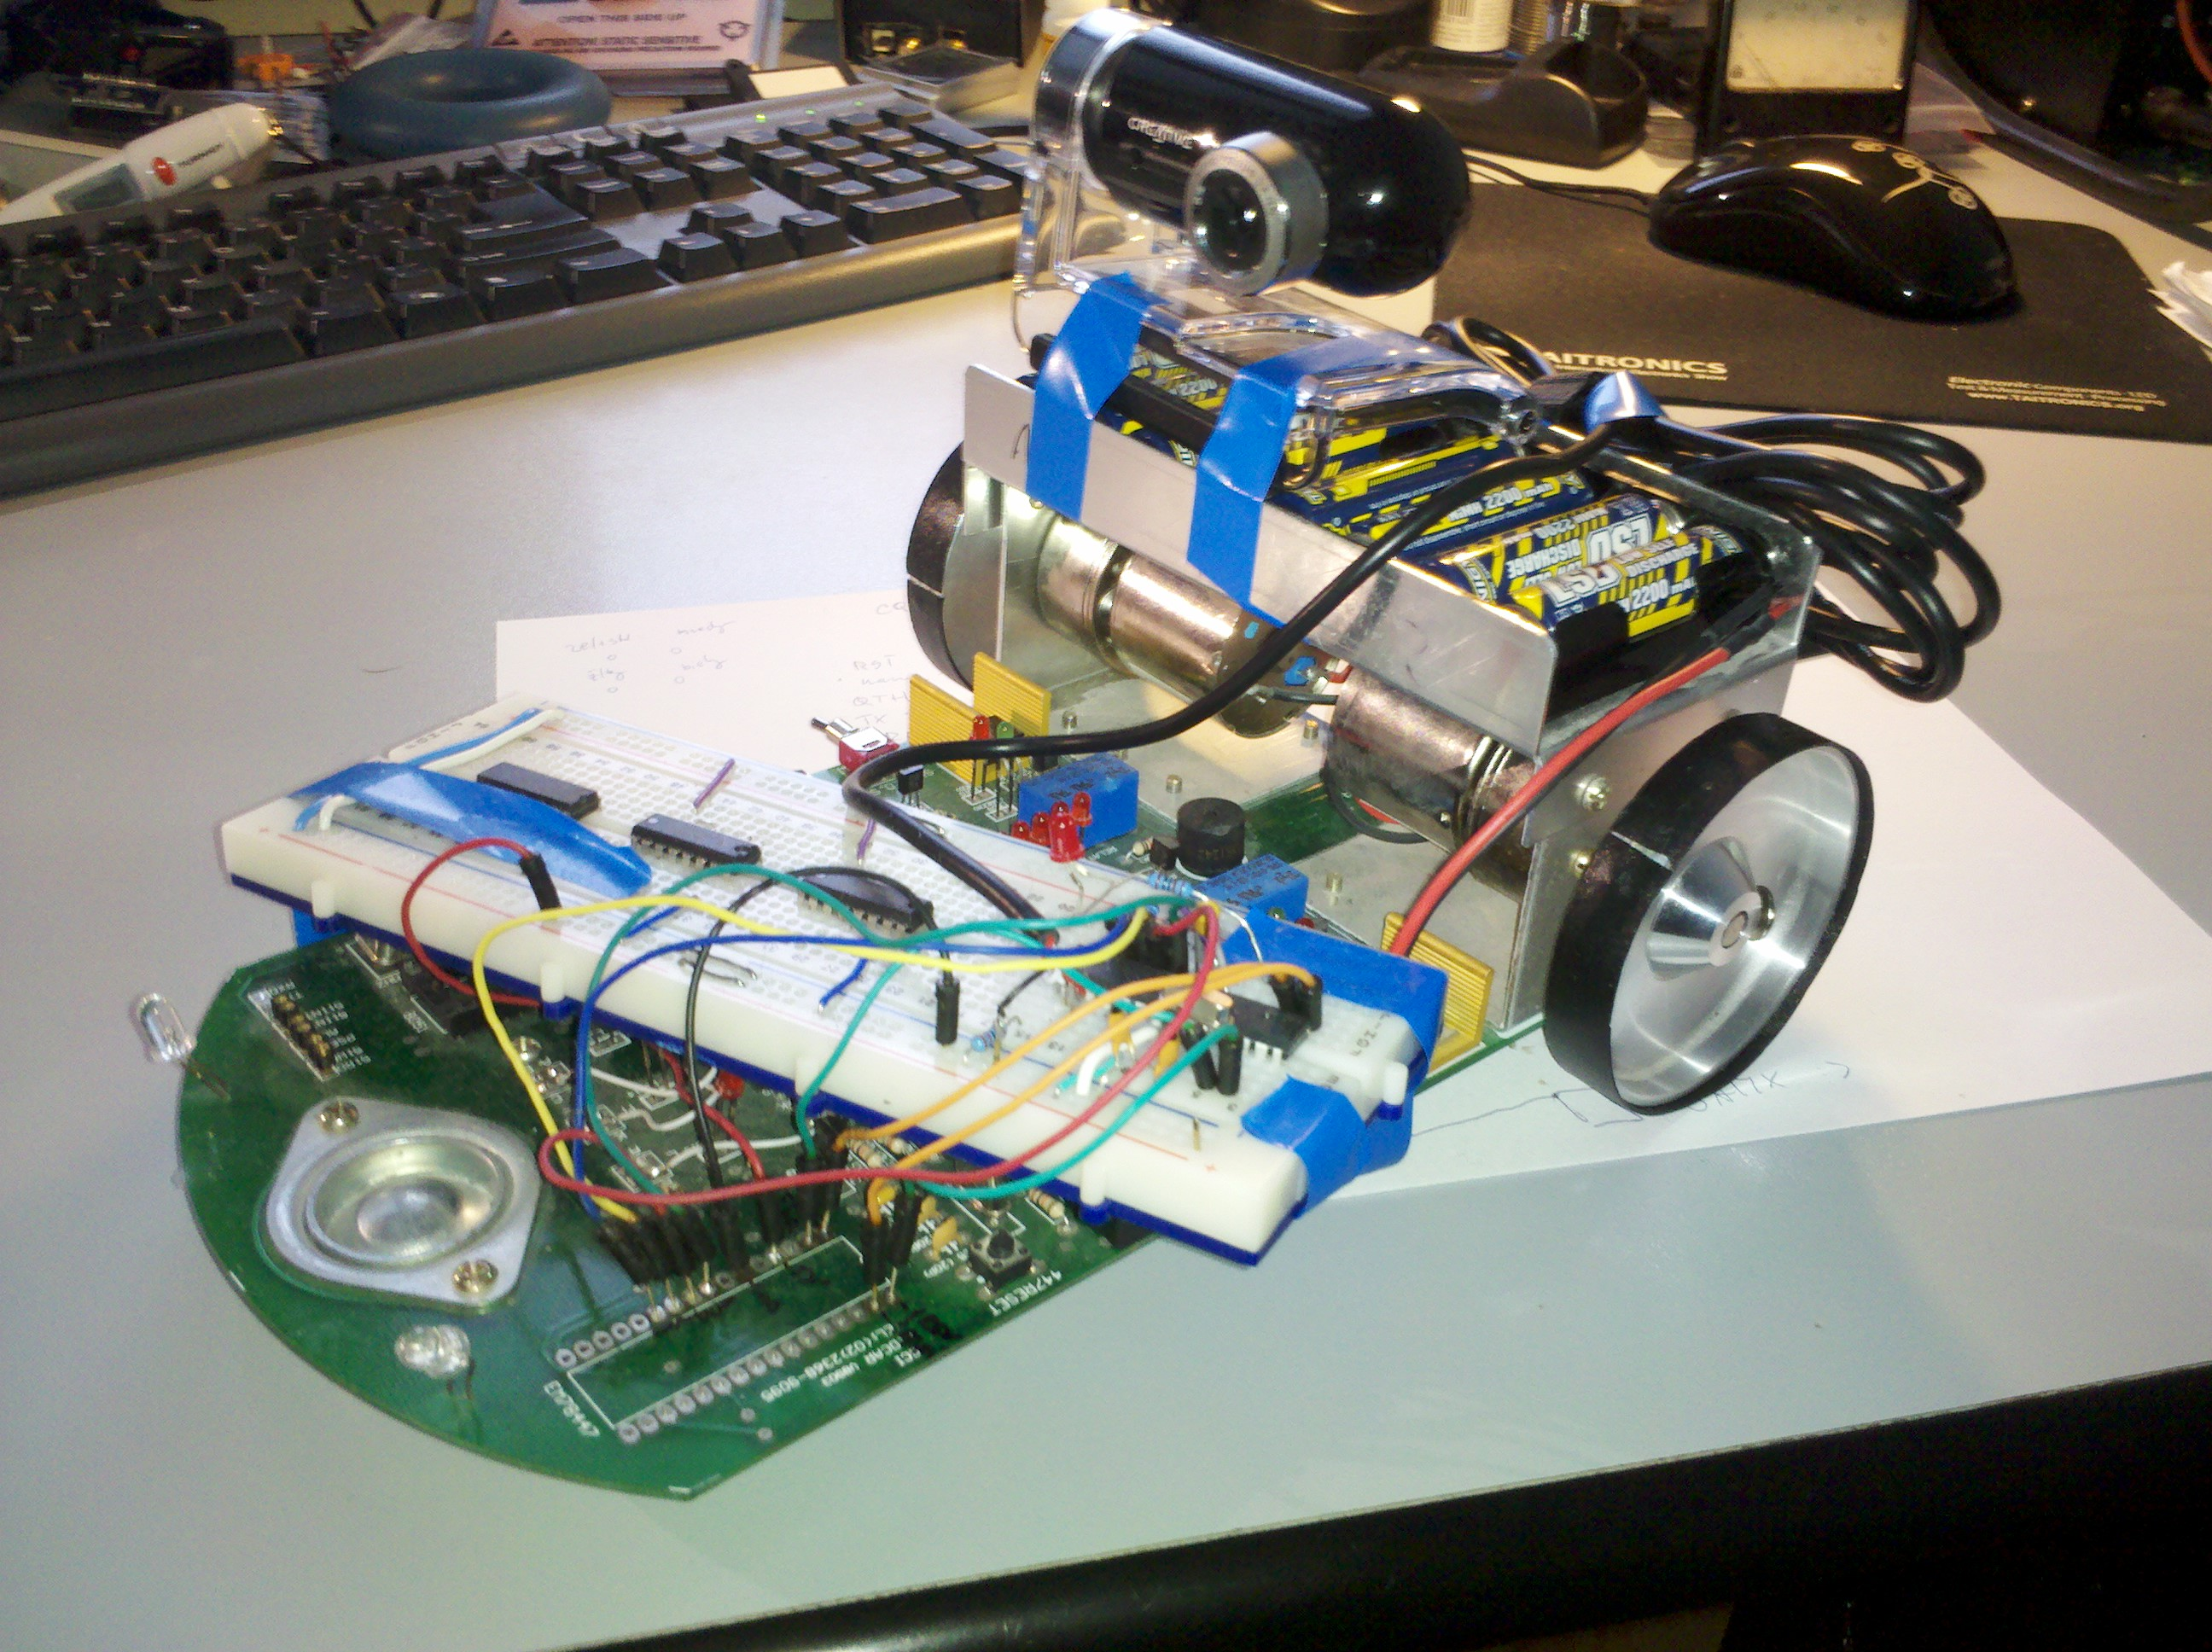
\includegraphics[width=1.05\paperwidth]{img1.jpg}
\end{centering}
\end{frame}

{
\setbeamercolor{background canvas}{bg=black,fg=white}
\usebeamercolor[fg]{background canvas}

\begin{frame}[plain]
\begin{centering}
\hspace{1.5cm}
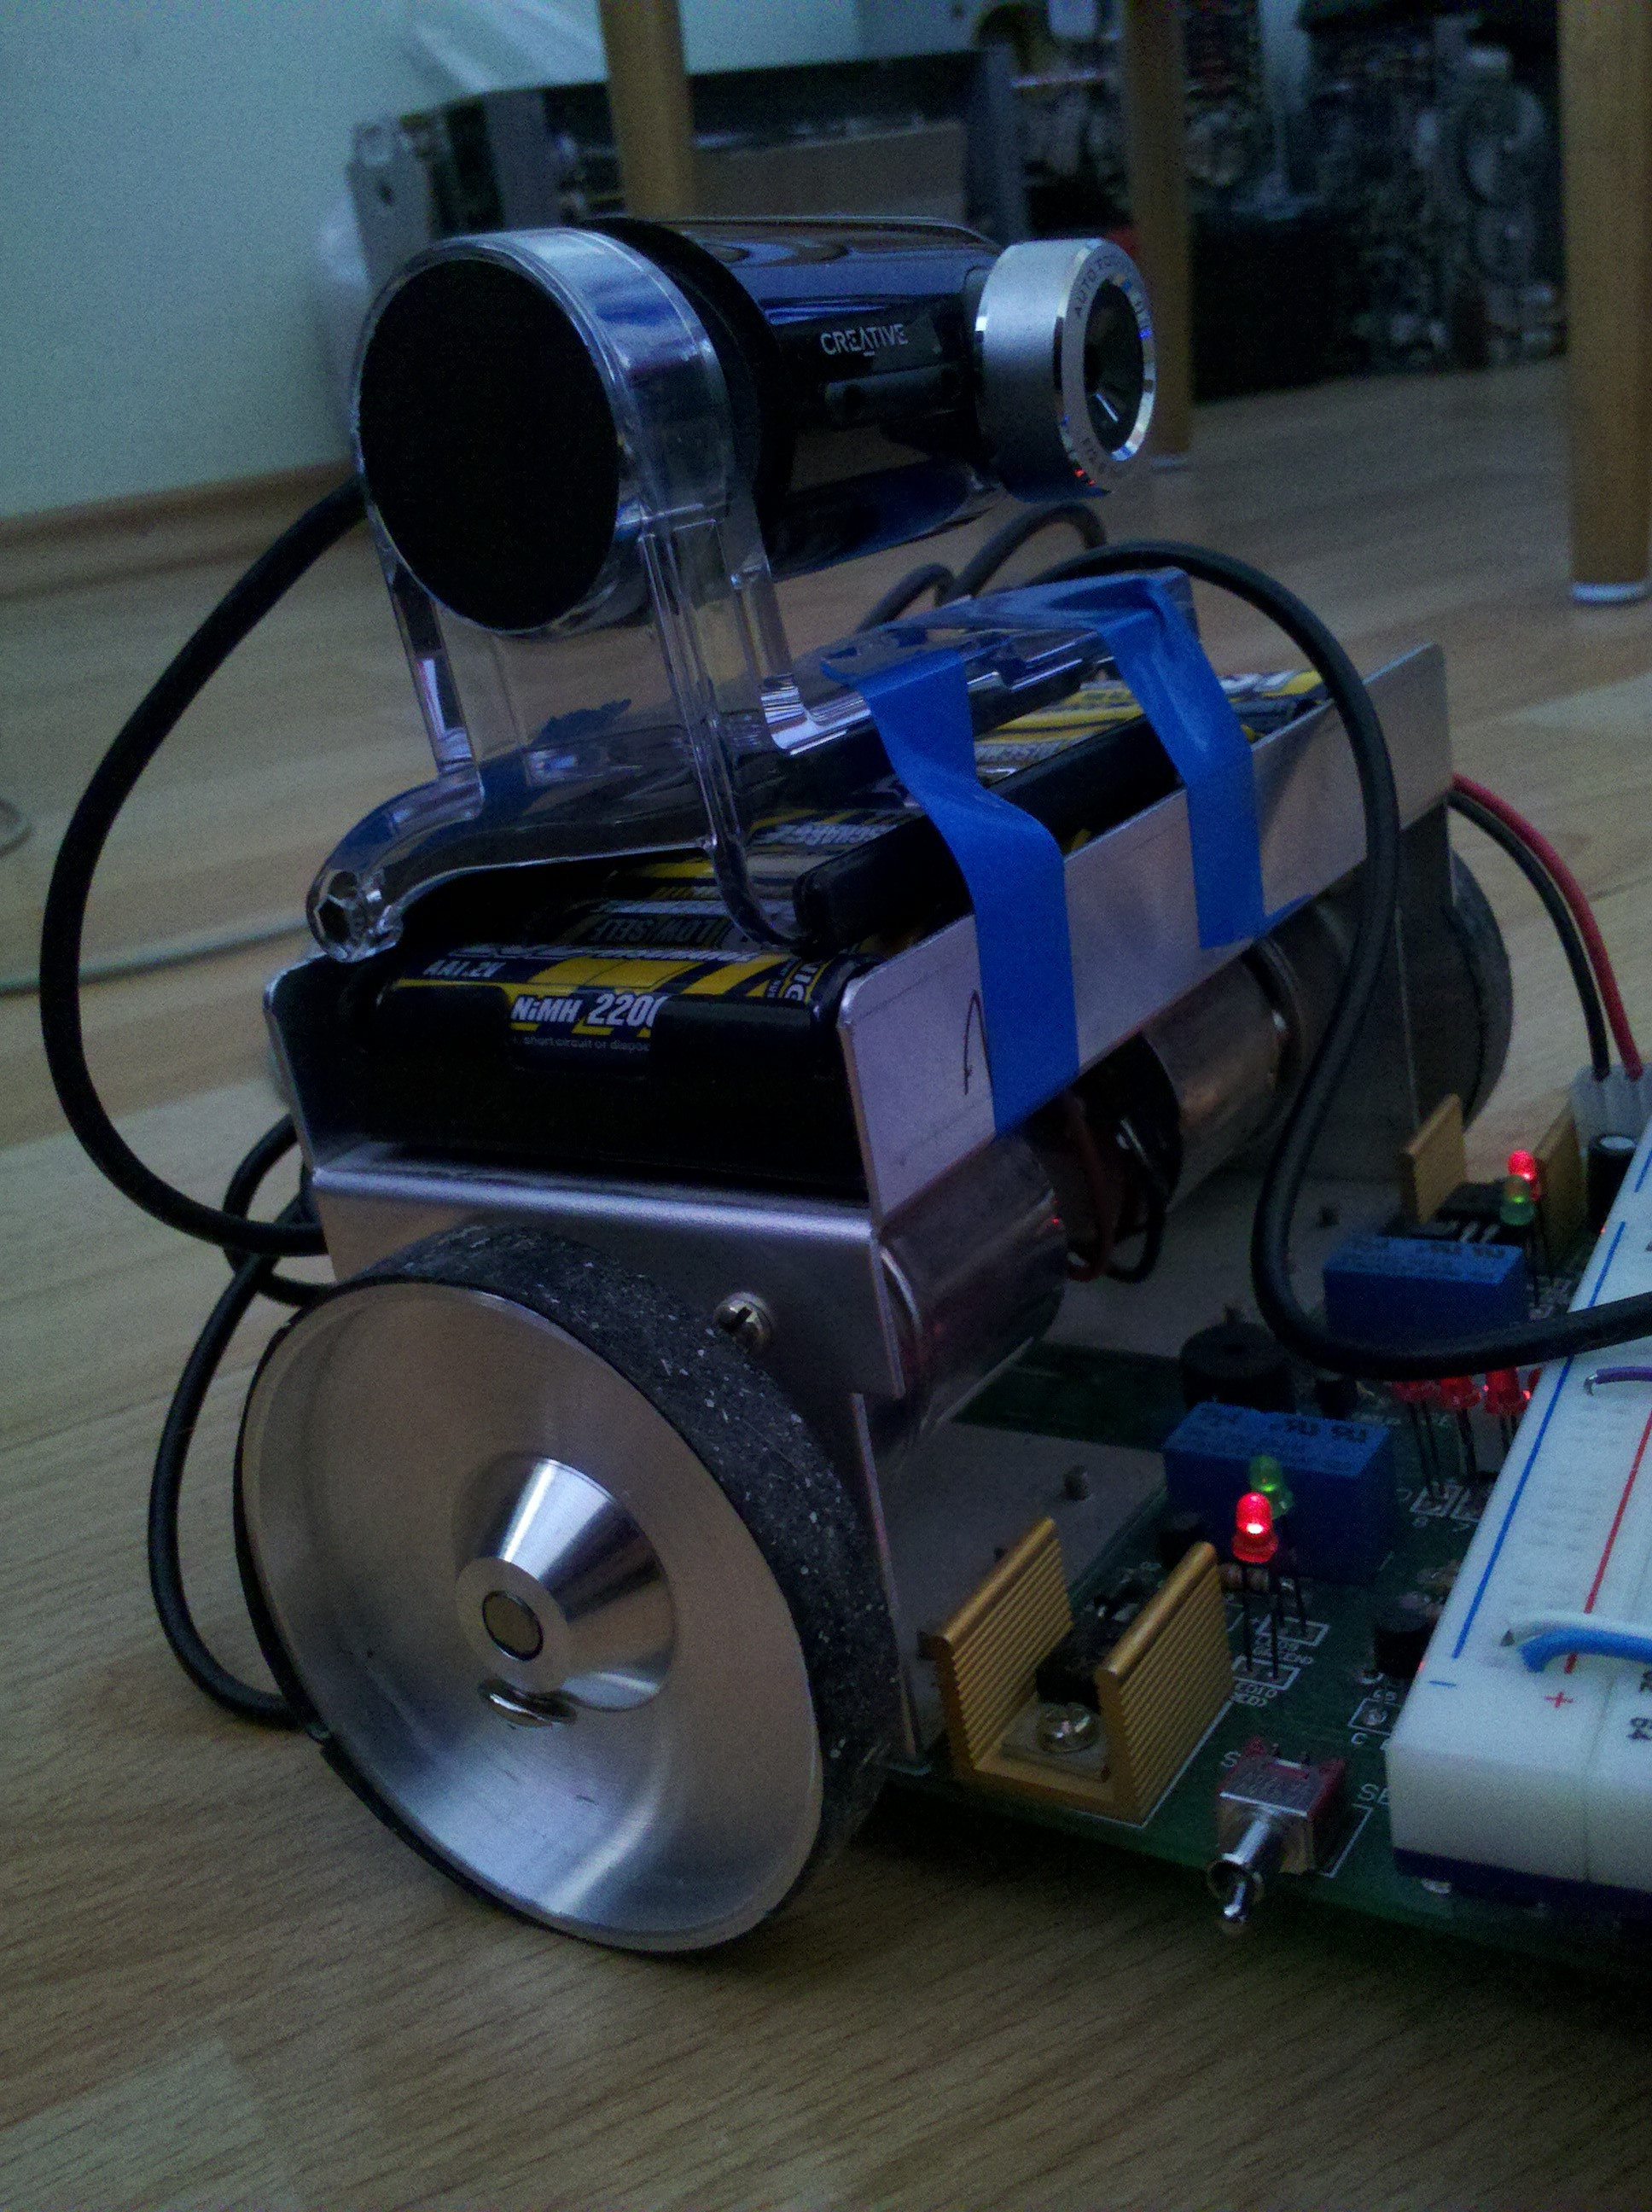
\includegraphics[height=1.05\paperheight]{img2.jpg}
\end{centering}
\end{frame}

}

\begin{frame}{Použité technologie}
\begin{itemize}
\item Nepoužili jsme Matlab!
\item FANN -- Fast Artificial Neural Network Library
\item OpenCV
\item 100 řádků C kódu pro $\mu{}C$
\item Pythonové skripty
\end{itemize}
\end{frame}

\begin{frame}{Části programu}
\begin{itemize}
\item record.py
	\begin{itemize}
	\item Nahrávání učících dat
	\end{itemize}
\item train.py
	\begin{itemize}
	\item Naučení sítě
	\end{itemize}
\item drive.py
	\begin{itemize}
	\item Jízda podle naučené sítě
	\end{itemize}
\end{itemize}
\end{frame}

\begin{frame}{Nahrávání}
\begin{itemize}
\item Obraz z kamery
\item Převod na ČB
\item Motion vektory
	\begin{itemize}
	\item OpenCV
	\item Block matching -- podobně jako MPEG
	\end{itemize}
\item Uložení spolu s vstupy joysticku
\end{itemize}
\end{frame}

\begin{frame}{Učení}
\begin{itemize}
\item Vyrovnání zpoždění obrazu
\item Vytvoření zrcadlových dat
\item Spojení více nahrávek do jedné
\item Učení sítě
	\begin{itemize}
	\item Learning rate: 0.2
	\item Algoritmus: quickprop
	\end{itemize}
\end{itemize}
\end{frame}

\begin{frame}{Neuronová síť}
\begin{itemize}
\item Dopředná neuronová síť
\item Vstupní vrstva: 108 neuronů
	\begin{itemize}
	\item 9 x 6 2D motion vektorů
	\end{itemize}
\item Skrytá vrstva: 32 neuronů
\item Výstupní vrstva: 2 neurony
	\begin{itemize}
	\item Rychlost
	\item Zatáčení
	\end{itemize}
\item Přenosová funkce: gaussian symmetric
\end{itemize}
\end{frame}

{
\setbeamercolor{background canvas}{bg=black,fg=white}
\usebeamercolor[fg]{background canvas}

\begin{frame}[plain]
\begin{centering}
%\includemovie[poster]{\paperheight}{\paperwidth}{nn-filtered.avi}
Video!
\end{centering}
\end{frame}

}

\begin{frame}{Problémy}
\begin{itemize}
\item Žádná testovací množina
	\begin{itemize}
	\item Další senzory
	\item Simulátor
	\item Ne pomocí standardních nástrojů v NN knihovně
	\end{itemize}
\item Webkamera
	\begin{itemize}
	\item Pouze MJPEG, nebo raw bitmapy -- Řešení: OpenCV
	\item Zpoždění obrazu
	\item Nevhodný zorný úhel
	\item Automatické ostření
	\end{itemize}
\item Podvozek
	\begin{itemize}
	\item Podkluz -- Řešení: Pogumování koleček
	\item Nepřesné řízení a velká setrvačnost
	\end{itemize}
\end{itemize}
\end{frame}

\begin{frame}{Konkurence}
\begin{itemize}
\item \url{http://www.youtube.com/watch?v=DWNtsS2kZWs}
\end{itemize}
\end{frame}

\begin{frame}{Konec}
\begin{itemize}
\item Konec?
\end{itemize}
\end{frame}

\end{document}
